\documentclass[aspectratio=169]{beamer}

\usepackage[utf8]{inputenc}

\usepackage{amsfonts}
\usepackage{amsmath}
\usepackage{color}
\usepackage{listings}
\usepackage{tikz}
\usepackage{hyperref}
\usepackage{multicol}
\usepackage{appendixnumberbeamer}

\usetheme{Rochester}
\usecolortheme{beaver}

\addtobeamertemplate{navigation symbols}{}{%
    \usebeamerfont{footline}%
    \usebeamercolor[fg]{footline}%
    \hspace{1em}%
    \insertframenumber/\inserttotalframenumber
}

\lstloadlanguages{C++}
    \lstset{%
        language={C++},
        basicstyle=\ttfamily,
        keywordstyle=\color{blue},
        showstringspaces=false,
        escapechar={§},
        escapeinside=||
    }

\newif\iftransitions
% \transitionstrue
 \transitionsfalse

\newcommand{\cpause}{\iftransitions \pause \fi}

\newcommand{\cuncover}[2]{\iftransitions \uncover<#1>{#2} \else #2 \fi}

\newif\iffast
% \fasttrue

\title{Durable Integer Arithmetic}
% \subtitle{An Introduction to Custom Allocators}
\author{Andreas Weis}
\institute{Woven Planet}

\date{CppNow 2022}
\titlegraphic{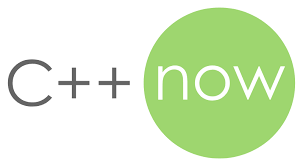
\includegraphics[height=.15\textheight]{resources/cppnow_logo.png}}

\iffalse
****************************** Abstract ******************************
Performing calculations on integers is one of the most fundamental tasks in any programming language. As such, the properties of integer arithmetic are often taken for granted. In this talk we will take a step back and re-evaluate how integer arithmetic is handled in C++.

We will start by taking a look at how integer arithmetic is commonly performed in hardware and how that differs from the rules used by the C++ language. We will then identify certain areas where the language rules turn out to be problematic, in particular for authors of numerical libraries. This will lead us to a more durable form of integer arithmetic. We will discuss hypothetical implementations of such a durable arithmetic on both language and library levels and explore the implications for numerical applications such as rational numbers, arbitrary precision integers and safe integers. We will look at some of the challenges that an implementation will have to overcome to enable efficient code generation and give an overview of how WG21 tries to address these challenges in some of its current proposals.
**********************************************************************
Submitted for onsite only.
**********************************************************************
Type: lecture
Level: Intermediate, Advanced, Expert
Audience: library authors, language designers, developers of numerical applications
****************************** Outline *******************************
- A brief recap of integer arithmetic
-- Addition of integers
-- Two's complement
-- Multiplication and Division
- Integer arithmetic in hardware vs. C/C++
- Examples of problematic behavior for library authors
-- Safe Integers (such as Boost.Safe Numerics)
-- Multi-precision Integers (such as Boost.Multiprecision)
-- Rational Numbers (such as Boost.Rational)
- Properties of a durable integer arithmetic
- Implementing durable integers as a library (*)
-- Correctness, Performance, Application
- Implementing durable integers as a language feature (*)
- Current proposals in WG21 (SG6)

* The two parts about implementation will be the guts of the presentation. The other sections are really a preliminary to understand the problem, but these two points are were the interesting questions get addressed and presumable were most of the discussions will take place. As such, they will also take up a major part of the time.
\fi

\begin{document}

\frame{\titlepage}

%\iftrue %crop

\begin{frame}[fragile]
  \frametitle{About me - Andreas Weis (he/him)}

  \begin{itemize}
    \setlength\itemsep{1.5em}

    \item \href{https://stackoverflow.com/users/577603/comicsansms}{
\includegraphics[height=.05\textheight]{resources/so-icon.png}} \href{https://github.com/ComicSansMS}{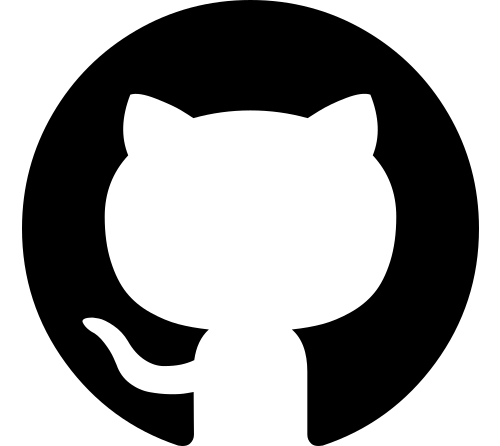
\includegraphics[height=.05\textheight]{resources/github-icon.png}} \includegraphics[height=.05\textheight]{resources/discord-icon.png} ComicSansMS

    \item \href{https://twitter.com/DerGhulbus/}{
\includegraphics[height=.05\textheight]{resources/twitter-icon.png} @DerGhulbus}

    \item 
\includegraphics[height=.05\textheight]{resources/meetup-icon.png} Co-organizer of the \href{https://www.meetup.com/MUCplusplus/}{Munich C++ User Group}

    \item Currently working as a Runtime Engineer for Woven Planet 
\includegraphics[height=.1\textheight]{resources/Woven_Planet_Holdings_Logo.png}

  \end{itemize}
\end{frame}


\begin{frame}
  \frametitle{Overview}
  \begin{itemize}
  \item A brief recap of integer arithmetic and their implementation in hardware
  \item Advanced use cases for integers in software
  \item Implementations of integer arithmetic in programming languages
  \item Expanding the capabilities of integer arithmetic in C++ through
  \begin{itemize}
    \item A third-party library
    \item The standard library
    \item A core language extension
  \end{itemize}
  \end{itemize}
\end{frame}

\begin{frame}
  \frametitle{Disclaimer}
  
  \begin{itemize}
  \item I am neither a professional mathematician nor a numerics expert
  \item I have put some thought into the presented designs, but way less than others, so be encouraged to challenge everything that I say
  \item The notation used in the math segments is heavily overloaded and hand-wavy. Please ask if the context of an equation is unclear to you
  \end{itemize}
\end{frame}

\begin{frame}
  \frametitle{Integer Arithmetic in Hardware}
  
  No C++, just hardware (for now)
\end{frame}

\begin{frame}
  \frametitle{Binary Representation of Integers}
  
  \begin{center}
  \Huge
  \only<1>{
  \begin{equation*}
  [1010]_2
  \end{equation*}
  }
  \only<2>{
  \begin{equation*}
  [\textcolor{purple}{1010}]_2
  \end{equation*}
  }
  \uncover<2>{
  \begin{equation*}
  = \textcolor{purple}{0} \times 2^0 + \textcolor{purple}{1} \times 2^1 + \textcolor{purple}{0} \times 2^2 + \textcolor{purple}{1} \times 2^3
  \end{equation*}
  }
  \end{center}
  
  Positional numeral system with base $B=2$.
\end{frame}

\begin{frame}
  \frametitle{Integer Addition}
  
  $0010 + 0111 = 1001$
  \begin{equation*}
    \begin{array}{c}
    \phantom{+9}0010\\
    +\phantom{9}0111 \\
    \underline{C\phantom{9}11\phantom{99}} \\
    \phantom{+}\phantom{9}1001
    \end{array}
  \end{equation*}
  
  $1101 + 1011 = \textcolor{red}{1}'1000$
  \begin{equation*}
    \begin{array}{c}
    \phantom{+9}1101\\
    +\phantom{9}1011 \\
    \underline{C1111\phantom{9}} \\
    \phantom{+}\textcolor{red}{1}1000
    \end{array}
  \end{equation*}
\end{frame}

\begin{frame}
  \frametitle{Addition in Hardware}
  
  \begin{columns}
    \begin{column}{.5\textwidth}
  
    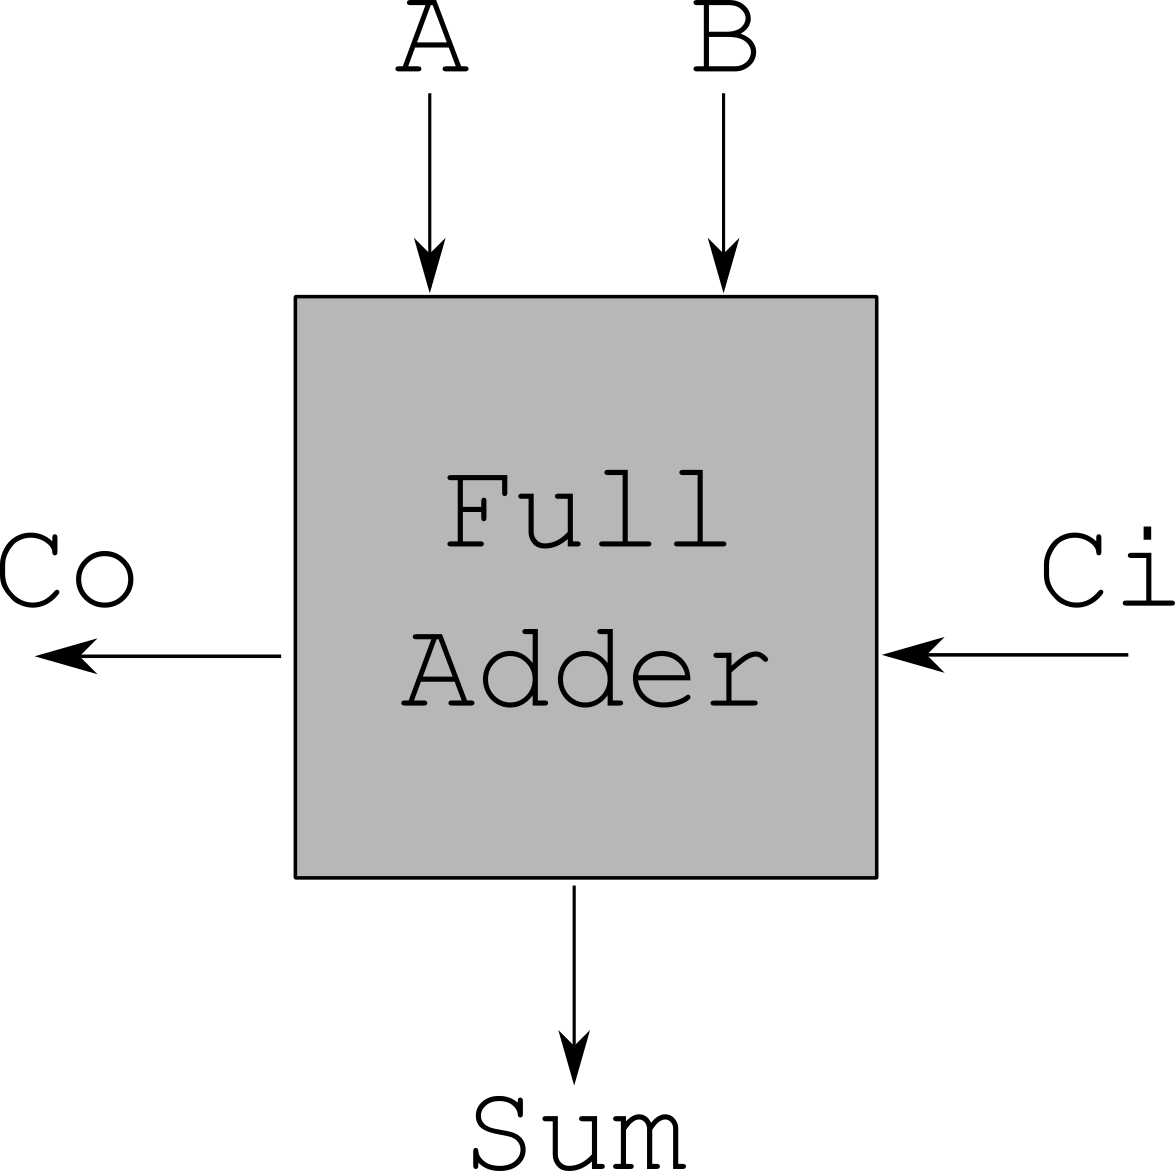
\includegraphics[width=.95\textwidth]{arithgfx/full_adder.png}
    \end{column}
    
    \begin{column}{.5\textwidth}
      \begin{tabular}{c c c|c c}
      A & B & Ci & Sum & Co \\
      \hline
      $0$ & $0$ & $0$ & $0$ & $0$ \\
      $0$ & $1$ & $0$ & $1$ & $0$ \\
      $1$ & $0$ & $0$ & $1$ & $0$ \\
      $1$ & $1$ & $0$ & $0$ & $1$ \\
      $0$ & $0$ & $1$ & $1$ & $0$ \\
      $0$ & $1$ & $1$ & $0$ & $1$ \\
      $1$ & $0$ & $1$ & $0$ & $1$ \\
      $1$ & $1$ & $1$ & $1$ & $1$ \\
      \end{tabular}
    \end{column}
  \end{columns}
\end{frame}

\begin{frame}
  \frametitle{Addition in Hardware}
  
  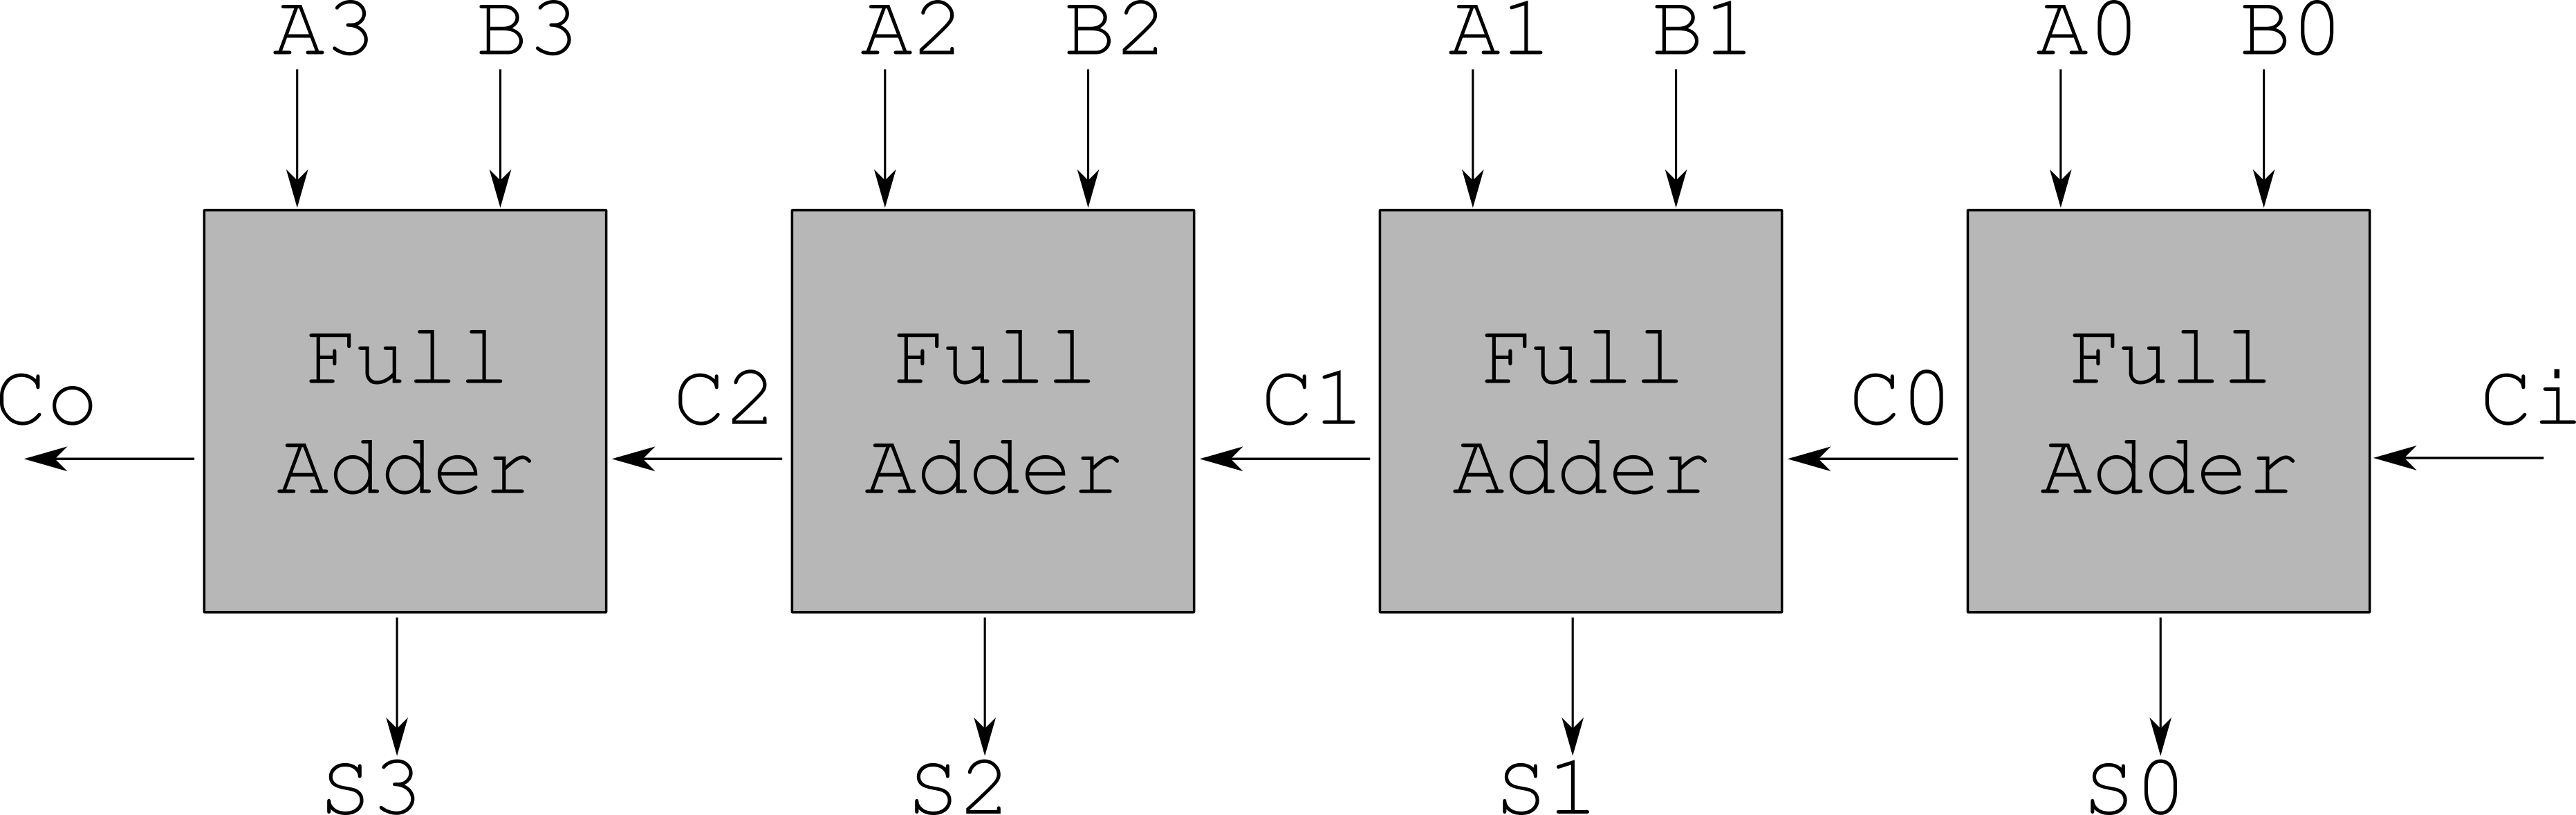
\includegraphics[width=.95\textwidth]{arithgfx/adder_ripple_carry.png}
\end{frame}

\begin{frame}
  \frametitle{Properties of Addition}
  \begin{itemize}
  \item Sum of two numbers with $n$ digits in base $B$ is representable as a number $B^n$ plus a carry bit
  \item $B^n + B^n = 2 \times B^n$ \iftransitions \pause \fi 
  \item The hardware implementation of the operation has no preconditions \iftransitions \pause \fi 
  \item Discarding the carry bit will lead to wrap-around ($\bmod B^n$)   \iftransitions \pause \fi 
  \item Most hardware implementations signal overflow via flag            \iftransitions \pause \fi 
  \item According for the carry bit by adding an additional digit to the result gives correct result in all cases
  \end{itemize}
\end{frame}


\begin{frame}
  \frametitle{Negative Integers and Two's Complement}
  
  \begin{itemize}
  \item Two's complement allows signed computations to be carried out using unsigned arithmetic
  \iftransitions
  \uncover<2->{ \item Inverting the sign of a number $x$ is done by calculating $-x = B^n - 1 - x + 1$ }
  \else
  \item Inverting the sign of a number $x$ is done by calculating $-x = B^n - 1 - x + 1$
  \fi
  \end{itemize}
  
  \begin{multicols}{2}
  \begin{equation*}\begin{array}{c}
   \phantom{999}0101\\
   \underline{\lnot\phantom{99}1010} \\
   \underline{+ \phantom{90}0001} \\
   \phantom{+99}1011
  \end{array}\end{equation*}
  
  \iftransitions \pause \fi 
  
  \begin{equation*}\begin{array}{c}
   \phantom{-99}1111 \\
   \underline{-\phantom{99}0101} \\
   \underline{\phantom{-99}1010} \\
   \underline{+ \phantom{90}0001} \\
   \phantom{+99}1011
  \end{array}\end{equation*}
  \end{multicols}
  
  
  
\end{frame}

\begin{frame}
  \frametitle{Negative Integers and Two's Complement}
  
  \only<1>{
  \begin{tabular}{l c c|l c c|l c c|l c c}
  Bin & Dec & \phantom{TC} & Bin & Dec & \phantom{TC} & Bin & Dec & \phantom{TC} & Bin & Dec & \phantom{TC} \\
  $0000$ & $ 0$ & \phantom{$0$} & $0100$ & $ 4$ & \phantom{$4$} & $1000$ & $ 8$ & \phantom{$-8$} & $1100$ & $12$ & \phantom{$-4$} \\
  $0001$ & $ 1$ & \phantom{$1$} & $0101$ & $ 5$ & \phantom{$5$} & $1001$ & $ 9$ & \phantom{$-7$} & $1101$ & $13$ & \phantom{$-3$} \\
  $0010$ & $ 2$ & \phantom{$2$} & $0110$ & $ 6$ & \phantom{$6$} & $1010$ & $10$ & \phantom{$-6$} & $1110$ & $14$ & \phantom{$-2$} \\
  $0011$ & $ 3$ & \phantom{$3$} & $0111$ & $ 7$ & \phantom{$7$} & $1011$ & $11$ & \phantom{$-5$} & $1111$ & $15$ & \phantom{$-1$} \\
  \end{tabular}
  }
  
  \only<2>{
  \begin{tabular}{l c c|l c c|l c c|l c c}
  Bin & Dec & TC & Bin & Dec & TC & Bin & Dec & TC & Bin & Dec & TC \\
  $0000$ & $ 0$ & $0$ & $0100$ & $ 4$ & $4$ & $1000$ & $ 8$ & $\textcolor{red}{-8}$ & $1100$ & $12$ & $\textcolor{red}{-4}$ \\
  $0001$ & $ 1$ & $1$ & $0101$ & $ 5$ & $5$ & $1001$ & $ 9$ & $\textcolor{red}{-7}$ & $1101$ & $13$ & $\textcolor{red}{-3}$ \\
  $0010$ & $ 2$ & $2$ & $0110$ & $ 6$ & $6$ & $1010$ & $10$ & $\textcolor{red}{-6}$ & $1110$ & $14$ & $\textcolor{red}{-2}$ \\
  $0011$ & $ 3$ & $3$ & $0111$ & $ 7$ & $7$ & $1011$ & $11$ & $\textcolor{red}{-5}$ & $1111$ & $15$ & $\textcolor{red}{-1}$ \\
  \end{tabular}
  }
\end{frame}

\begin{frame}
  \frametitle{Subtraction}
  
  \begin{equation*}
    a - a = a + (-a) = a + (2^n - 1 - a + 1)
  \end{equation*} \iftransitions \pause \fi 
  \begin{equation*}
    = a - a + 2^n - 1 + 1
  \end{equation*} \iftransitions \pause \fi 
  \begin{equation*}
    = 2^n \equiv 0 \bmod 2^n
  \end{equation*}
\end{frame}

\begin{frame}
  \frametitle{Subtraction}
  
  \begin{tabular}{l c c|l c c|l c c|l c c}
  Bin & Dec & TC & Bin & Dec & TC & Bin & Dec & TC & Bin & Dec & TC \\
  $0000$ & $ 0$ & $0$ & $0100$ & $ 4$ & $4$ & $1000$ & $ 8$ & $-8$ & $1100$ & $12$ & $-4$ \\
  $0001$ & $ 1$ & $1$ & $\textcolor{teal}{0101}$ & $ \textcolor{teal}{5}$ & $\textcolor{teal}{5}$ & $1001$ & $ 9$ & $-7$ & $1101$ & $13$ & $-3$ \\
  $0010$ & $ 2$ & $2$ & $0110$ & $ 6$ & $6$ & $1010$ & $10$ & $-6$ & $1110$ & $14$ & $-2$ \\
  $0011$ & $ 3$ & $3$ & $0111$ & $ 7$ & $7$ & $\textcolor{purple}{1011}$ & $\textcolor{purple}{11}$ & $\textcolor{purple}{-5}$ & $1111$ & $15$ & $-1$ \\
  \end{tabular}
  
  \vspace{20pt}

  \begin{equation*}\begin{array}{c}
   \phantom{+9}\textcolor{teal}{0101} \phantom{999-+/99} (5) \\
   \underline{+\phantom{9}\textcolor{purple}{1011}} \phantom{999} (-5/+11) \\
   \phantom{+}\textcolor{red}{1}0000 \phantom{999-+} (0/16)
  \end{array}\end{equation*}
\end{frame}


\begin{frame}
  \frametitle{Subtraction}
  
  \begin{equation*}
    a - b = a + (-b) = a + (2^n - 1 - b + 1)
  \end{equation*} \iftransitions \pause \fi 
  \begin{equation*}
    = a - b + 2^n - 1 + 1
  \end{equation*} \iftransitions \pause \fi 
  \begin{equation*}
    = a - b + 2^n \equiv a - b \bmod 2^n
  \end{equation*}
\end{frame}

\begin{frame}
  \frametitle{Subtraction}
  
  \begin{tabular}{l c c|l c c|l c c|l c c}
  Bin & Dec & TC & Bin & Dec & TC & Bin & Dec & TC & Bin & Dec & TC \\
  $0000$ & $ 0$ & $0$ & $0100$ & $ 4$ & $4$ & $1000$ & $ 8$ & $-8$ & $1100$ & $12$ & $-4$ \\
  $0001$ & $ 1$ & $1$ & $\textcolor{teal}{0101}$ & $\textcolor{teal}{ 5}$ & $\textcolor{teal}{ 5}$ & $1001$ & $ 9$ & $-7$ & $\textcolor{purple}{1101}$ & $\textcolor{purple}{13}$ & $\textcolor{purple}{-3}$ \\
  $0010$ & $ 2$ & $2$ & $0110$ & $ 6$ & $6$ & $1010$ & $10$ & $-6$ & $1110$ & $14$ & $-2$ \\
  $0011$ & $ 3$ & $3$ & $0111$ & $ 7$ & $7$ & $1011$ & $11$ & $-5$ & $1111$ & $15$ & $-1$ \\
  \end{tabular}
  
  \vspace{20pt}

  \begin{equation*}\begin{array}{c}
   \phantom{+9}\textcolor{teal}{0101} \phantom{999-+/99} (5) \\
   \underline{+\phantom{9}\textcolor{purple}{1101}} \phantom{999} (-3/+13) \\
   \phantom{+}\textcolor{red}{1}0010 \phantom{999-+} (2/18)
  \end{array}\end{equation*}
\end{frame}


\begin{frame}
  \frametitle{Subtraction}
  
  \begin{equation*}
    -a - b = (-a) + (-b) = (2^n - 1 - a + 1) + (2^n - 1 - b + 1)
  \end{equation*} \iftransitions \pause \fi 
  \begin{equation*}
    = -a - b + 2^n - 1 + 1 + 2^n - 1 + 1
  \end{equation*} \iftransitions \pause \fi 
  \begin{equation*}
    = -a - b + 2^{n+1} \equiv -a - b \bmod 2^n
  \end{equation*}
\end{frame}

\begin{frame}
  \frametitle{Subtraction}
  
  \begin{tabular}{l c c|l c c|l c c|l c c}
  Bin & Dec & TC & Bin & Dec & TC & Bin & Dec & TC & Bin & Dec & TC \\
  $0000$ & $ 0$ & $0$ & $0100$ & $ 4$ & $4$ & $1000$ & $ 8$ & $-8$ & $1100$ & $12$ & $-4$ \\
  $0001$ & $ 1$ & $1$ & $0101$ & $ 5$ & $5$ & $1001$ & $ 9$ & $-7$ & $\textcolor{purple}{1101}$ & $\textcolor{purple}{13}$ & $\textcolor{purple}{-3}$ \\
  $0010$ & $ 2$ & $2$ & $0110$ & $ 6$ & $6$ & $1010$ & $10$ & $-6$ & $1110$ & $14$ & $-2$ \\
  $0011$ & $ 3$ & $3$ & $0111$ & $ 7$ & $7$ & $\textcolor{teal}{1011}$ & $\textcolor{teal}{11}$ & $\textcolor{teal}{-5}$ & $1111$ & $15$ & $-1$ \\
  \end{tabular}
  
  \vspace{20pt}

  \begin{equation*}\begin{array}{c}
   \phantom{+9}\textcolor{teal}{1011} \phantom{999} (-5/+11) \\
   \underline{+\phantom{9}\textcolor{purple}{1101}} \phantom{999} (-3/+13) \\
   \phantom{+}\textcolor{red}{1}1000 \phantom{999} (-8/+24)
  \end{array}\end{equation*}
\end{frame}


\begin{frame}
  \frametitle{Carry and Overflow}
  
  \begin{multicols}{3}
  \begin{equation*}\begin{array}{c}
   \phantom{+9}0101 \phantom{999-+/99} (5) \\
   \underline{+\phantom{9}1011} \phantom{999} (-5/+11) \\
   \phantom{+}\textcolor{red}{1}0000 \phantom{999-+} (0/16)
  \end{array}\end{equation*} \iftransitions \pause \fi 
  
  \begin{equation*}\begin{array}{c}
   \phantom{+9}0101 \phantom{999-+/99} (5) \\
   \underline{+\phantom{9}1101} \phantom{999} (-3/+13) \\
   \phantom{+}\textcolor{red}{1}0010 \phantom{999-+} (2/18)
  \end{array}\end{equation*} \iftransitions \pause \fi 
  
  \begin{equation*}\begin{array}{c}
   \phantom{+9}1011 \phantom{999} (-5/+11) \\
   \underline{+\phantom{9}1101} \phantom{999} (-3/+13) \\
   \phantom{+}\textcolor{red}{1}1000 \phantom{999} (-8/+24)
  \end{array}\end{equation*} \iftransitions \pause \fi 
  \end{multicols}
  
  \begin{multicols}{2}
  \begin{equation*}\begin{array}{c}
   \phantom{+9}0101 \phantom{999-+/99} (5) \\
   \underline{+\phantom{9}0110} \phantom{999-+/99} (6) \\
   \phantom{+}\textcolor{red}{0}1011 \phantom{999-+/9} (11)
  \end{array}\end{equation*} \iftransitions \pause \fi 
  
  \begin{equation*}\begin{array}{c}
   \phantom{+9}1001 \phantom{999+/99} (-7) \\
   \underline{+\phantom{9}1010} \phantom{999+/99} (-6) \\
   \phantom{+}\textcolor{red}{1}0011 \phantom{999-+/9} (19)
  \end{array}\end{equation*}
  \end{multicols}
  
  \iftransitions \pause \fi
  
  \begin{itemize}
  \item Carry = Unsigned Overflow
  \item Overflow = Signed Overflow
  \end{itemize}
\end{frame}

\begin{frame}
  \frametitle{Properties of Subtraction}
  
  \begin{tabular}{l c c|l c c|l c c|l c c}
  Bin & Dec & TC & Bin & Dec & TC & Bin & Dec & TC & Bin & Dec & TC \\
  $0000$ & $ 0$ & $0$ & $0100$ & $ 4$ & $4$ & $1000$ & $ 8$ & $-8$ & $1100$ & $12$ & $-4$ \\
  $0001$ & $ 1$ & $1$ & $0101$ & $ 5$ & $5$ & $1001$ & $ 9$ & $-7$ & $1101$ & $13$ & $-3$ \\
  $0010$ & $ 2$ & $2$ & $0110$ & $ 6$ & $6$ & $1010$ & $10$ & $-6$ & $1110$ & $14$ & $-2$ \\
  $0011$ & $ 3$ & $3$ & $0111$ & $ 7$ & $7$ & $1011$ & $11$ & $-5$ & $1111$ & $15$ & $-1$ \\
  \end{tabular}
  
  
  \begin{itemize}
  \item Subtraction in two's complement is carried out using the same logic as unsigned addition  \iftransitions \pause \fi 
  \item Like unsigned addition, there are no preconditions  \iftransitions \pause \fi 
  \item The overflow condition changes; the unsigned carry flag has no meaningful semantics on its own for signed addition  \iftransitions \pause \fi 
  \item Because of the way that negative numbers are mapped onto the unsigned values, calculations overflowing \texttt{INT\_MAX} wrap around to \texttt{INT\_MIN}
  \end{itemize}
\end{frame}

\begin{frame}
  \frametitle{Multiplication}
  
  \begin{equation*}\begin{array}{c}
   \underline{\phantom{+}1001 \times 1101}\\
   \phantom{+}1 \times \phantom{999}1101\phantom{9} \\
   \textcolor{gray}{+0 \times \phantom{99}1101\phantom{99}} \\
   \textcolor{gray}{+0 \times \phantom{9}1101\phantom{999}} \\
   \underline{+ 1 \times 1101\phantom{9999}} \\
   \phantom{+ 11 \times }1110101\phantom{9}
  \end{array}\end{equation*}
\end{frame}

\begin{frame}
  \frametitle{Multiplication}
  
  \begin{equation*}\begin{array}{c}
   \underline{\phantom{+}1001 \times 1101}\\
   \phantom{+}1 \times \phantom{999}1101\phantom{9} \\
   \underline{+ 1 \times 1101\phantom{9999}} \\
   \phantom{+ 11 \times }1110101\phantom{9}
  \end{array}\end{equation*}
  
  \begin{itemize}
  \item Implemented in hardware as a series of shifts and additions \iftransitions \pause \fi 
  \item Works naturally for negative numbers in two's complement after sign extension
  \end{itemize}
\end{frame}

\begin{frame}
  \frametitle{Multiplication - Biggest Result}
  
  \begin{itemize}
  \item Product of two numbers $< B^n$ is  at most $B^n \times B^n = B^{2n}$
  \end{itemize}
  
  \iftransitions \pause \fi 
  
  \begin{equation*}\begin{array}{c}
   \underline{\phantom{+}1111 \times 1111}\\
   \phantom{+}1 \times \phantom{999}1111\phantom{9} \\
   +1 \times \phantom{99}1111\phantom{99} \\
   +1 \times \phantom{9}1111\phantom{999} \\
   \underline{+ 1 \times 1111\phantom{9999}} \\
   \phantom{+ 1 \times }\textcolor{red}{1110}0001\phantom{9}
  \end{array}\end{equation*}
  
\end{frame}

\begin{frame}
  \frametitle{Properties of Multiplication}
  
  \begin{itemize}
  \item Representing the full result of multiplication requires twice the number of digits of the input  \iftransitions \pause \fi 
  \item Overflow occurs when the upper half of the result is not $0$  \iftransitions \pause \fi 
  \item Like addition, hardware implementations of multiplication have no preconditions and overflow is typically reported via flag  \iftransitions \pause \fi 
  \item Hardware architectures typically provide single and double-width forms of multiplication
  \end{itemize}
\end{frame}

\begin{frame}
  \frametitle{Division}
  
  \begin{itemize}
  \item Division is significantly more complicated than the other operations  \iftransitions \pause \fi 
  \item $+$, $-$, $\times$ are all primitive operations in VHDL/Verilog, division is often coded explicitly  \iftransitions \pause \fi 
  \item Division circuits often introduce $n^2$ delays and are usually slow to execute  \iftransitions \pause \fi 
  \item Like with long division, the remainder is naturally computed as part of hardware division  \iftransitions \pause \fi 
  \item Signed division can overflow, but only in corner cases
  \end{itemize}
\end{frame}

\begin{frame}
  \frametitle{Preconditions of Division}
  
  \begin{itemize}
  \item Unlike the other basic operations, division has a precondition -- the divisor must be $\neq 0$  \iftransitions \pause \fi 
  \item This is due to $0$ being an absorbing element of multiplication  \iftransitions \pause \fi 
  \item There is no meaningful extension to algebra of natural numbers in which division by 0 has a meaningful result; such extensions do exist for rational and real numbers though  \iftransitions \pause \fi 
  \item Hardware typically traps on division by 0
  \end{itemize}
\end{frame}

\begin{frame}
  \frametitle{Hardware Summary}
  
  \begin{itemize}
  \item Behaviour of elemental operations is well-defined for all inputs (except division~by~$0$)
  \item Overflow conditions are typically signaled through flags
  \item All operations can be carried out without loss of information for arbitrary inputs
  \item Computing the quotient of two numbers gives the remainder for free
  \end{itemize}

\end{frame}

\begin{frame}
  \frametitle{Use Case: Safe Integers}
  
  \begin{itemize}
    \item Integer overflow (signed and unsigned) is almost always a bug
    \item Safe integer calculations detect overflow conditions and prohibit using the results
    \item Overflow checks are difficult to carry out correctly when overflow is undefined behavior
    \item Vital use case for domains that require high reliability
  \end{itemize}
\end{frame}

\begin{frame}
  \frametitle{Use Case: Arbitrary Precision Arithmetic \& Big Numbers}
  
  \begin{itemize}
    \item Naïve implementation just stores a list of bits and performs calculations bitwise in software
    \item Algorithms on positional calculations work for arbitrary bases
    \item More efficient implementation carries out calculations in chunks of machine word widths
    \item Overflow of less significant chunks carries over to more significant chunks
    \item Hardware sometimes provides special instructions for this use case (e.g. add-with-carry)
  \end{itemize}
\end{frame}


\begin{frame}
  \frametitle{Use Case: Rational Number Arithmetic}
  
  \begin{itemize}
    \item Rational arithmetic is more exact than floating point arithmetic for certain values
    \item Like IEEE-754 floats, rational arithmetic can be extended with special values to handle division~by~$0$, thereby allowing all fundamental operations with no preconditions
    \item $\frac{x}{0} \rightarrow \infty$, $-\frac{x}{0} \rightarrow -\infty$, $\frac{0}{0} \rightarrow NaN$; but is this a meaningful extension?
    \item To stay consistent with IEEE-754:
        \begin{quotation}
        The behavior of infinity in floating-point arithmetic is derived from the limiting cases of real arithmetic with
operands of arbitrarily large magnitude, when such a limit exists. 
        \end{quotation}
  \end{itemize}
\end{frame}

\begin{frame}
  \frametitle{Calculating with Rational Numbers}
  
  \begin{equation*}
  e^x = 1+ x + \frac{x^2}{2!} + \frac{x^3}{3!} + \frac{x^4}{4!} + \ldots = \sum_{n = 0}^{\infty}{\frac{x^{n}}{n!}}
  \end{equation*}
  \iftransitions \pause \fi 
  
  Calculating $e^1$ and $e^3$
  \begin{tabular}{c c c c c}
  \#iter & $e^1$ & float & $(e^1)^3$ & float   \\
  $2$ & $\frac{5   }{2   }$ & $2.5000000000000000$ &  $\frac{125}{8}$              & $15.625000000000000$ \\[5pt]
  $3$ & $\frac{8   }{3   }$ & $2.6666666666666665$ &  $\frac{512}{27}$             & $18.962962962962962$ \\[5pt]
  $4$ & $\frac{65  }{24  }$ & $2.7083333333333335$ &  $\frac{274625}{13842}$       & $19.865813078703702$ \\[5pt]
  $5$ & $\frac{163 }{60  }$ & $2.7166666666666668$ &  $\frac{4330747}{216000}$     & $20.049754629629629$ \\[5pt]
  $6$ & $\frac{1957}{720 }$ & $2.7180555555555554$ &  Overflow!                    & ---                  \\[5pt]
  $7$ & $\frac{685 }{252 }$ & $2.7182539682539684$ &  $\frac{321419125}{16003008}$ & $20.084919347662641$ \\[5pt]
  \end{tabular}
\end{frame}

\begin{frame}
  \frametitle{Durable Integer Arithmetic}
  
  \begin{itemize}
  \item Solving these (and other) use cases of integer arithmetic is difficult with the built-in integer types  \iftransitions \pause \fi 
  \item Hardware instructions were designed to be flexible enough to handle them, but this flexibility is lost in the abstractions of higher-level languages  \iftransitions \pause \fi 
  \item Instead of thinking about how to provide libraries for specific use cases, instead consider how to expose the semantics of the hardware instruction to those who need it
  \end{itemize}
\end{frame}

\begin{frame}
  \frametitle{Implementation in Programming Languages}
  
  ISO/IEC 10967:1 (2012) - Language Independent Arithmetic: Integer and Floating Point Arithmetic
  
  \begin{itemize}
  \item Worked out by the (now disbanded) SC22/WG11 - Binding Techniques  \iftransitions \pause \fi 
  \item Mandates the modeling of error states such as overflow as exceptional values in the return type of computations  \iftransitions \pause \fi 
  \item Does not specify double-width operations  \iftransitions \pause \fi 
  \item Has never been implemented anywhere?
  \end{itemize}
\end{frame}

\begin{frame}
  \frametitle{Implementation in C and C++}
  
  For built-in integer types:
  \begin{itemize}
  \item Signed overflow and division by zero are undefined behavior  \iftransitions \pause \fi 
  \item Historically, this was not always the case! \iftransitions \pause \fi 
  \item Compilers optimize heavy on this; for instance performing addition using opcodes that don't set flags  \iftransitions \pause \fi 
  \item Integer types are subject to arcane conversion rules during computation  \iftransitions \pause \fi 
  \item Compilers often optimize double-width division, but not double-width multiplication \iftransitions \pause \fi 
  \end{itemize}
  
  These were good defaults in the 1970s, but they are very limiting today.
  
  Changes to the behavior of the built-in operations are unlikely to happen ever.
\end{frame}

\begin{frame}
  \frametitle{Implementation in younger languages}
  
  \begin{itemize}
    \item Go
    \begin{itemize}
      \item Silently wraps on signed overflow
      \item No standard library support for checked or double width operations.
    \end{itemize}  \iftransitions \pause \fi 
    \item Rust
    \begin{itemize}
      \item Panic on signed overflow in debug and wrap in release
      \item Provides library functions for checked arithmetic
      \item Double width multiply with carry input, but no division
    \end{itemize}    \iftransitions \pause \fi 
    \item Swift 
    \begin{itemize}
      \item Overflow is an error by default, provides special operators for wrap
      \item Provides library functions for checked arithmetic
      \item Provides double width multiply and divide, but no carry input
    \end{itemize}
  \end{itemize}

\end{frame}

\begin{frame}
  \frametitle{Can we get this for C++?}

  What I would like to get:
  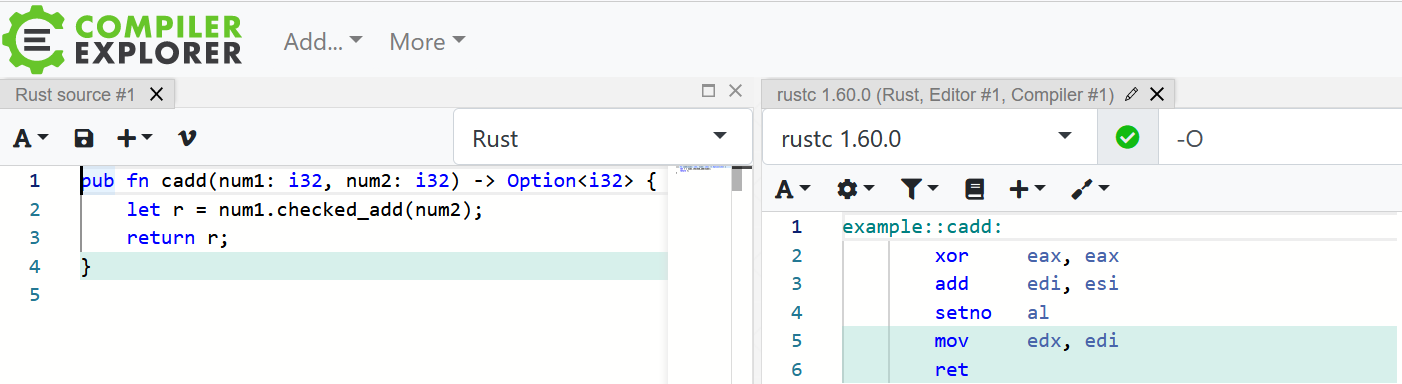
\includegraphics[width=.95\textwidth]{arithgfx/rust_add.png}
\end{frame}

\begin{frame}
  \frametitle{Can we get this for C++?}

  \begin{itemize}
    \item Goal is to provide a minimal set of fundamental operations that map closely to the operations provided by hardware  \iftransitions \pause \fi 
    \item These operations serve as building blocks for more powerful abstractions  \iftransitions \pause \fi 
    \item Users are unlikely to use them directly, but they enable library developers to solve relevant use cases  \iftransitions \pause \fi 
    \item Instead of having to wait for a library that solves each problem, enables developers to solve problems on their own if they need to
  \end{itemize}
\end{frame}

\begin{frame}
  \frametitle{Attempt \#1: Rely on the compiler to optimize it for us}

  \iftransitions \pause \fi 
  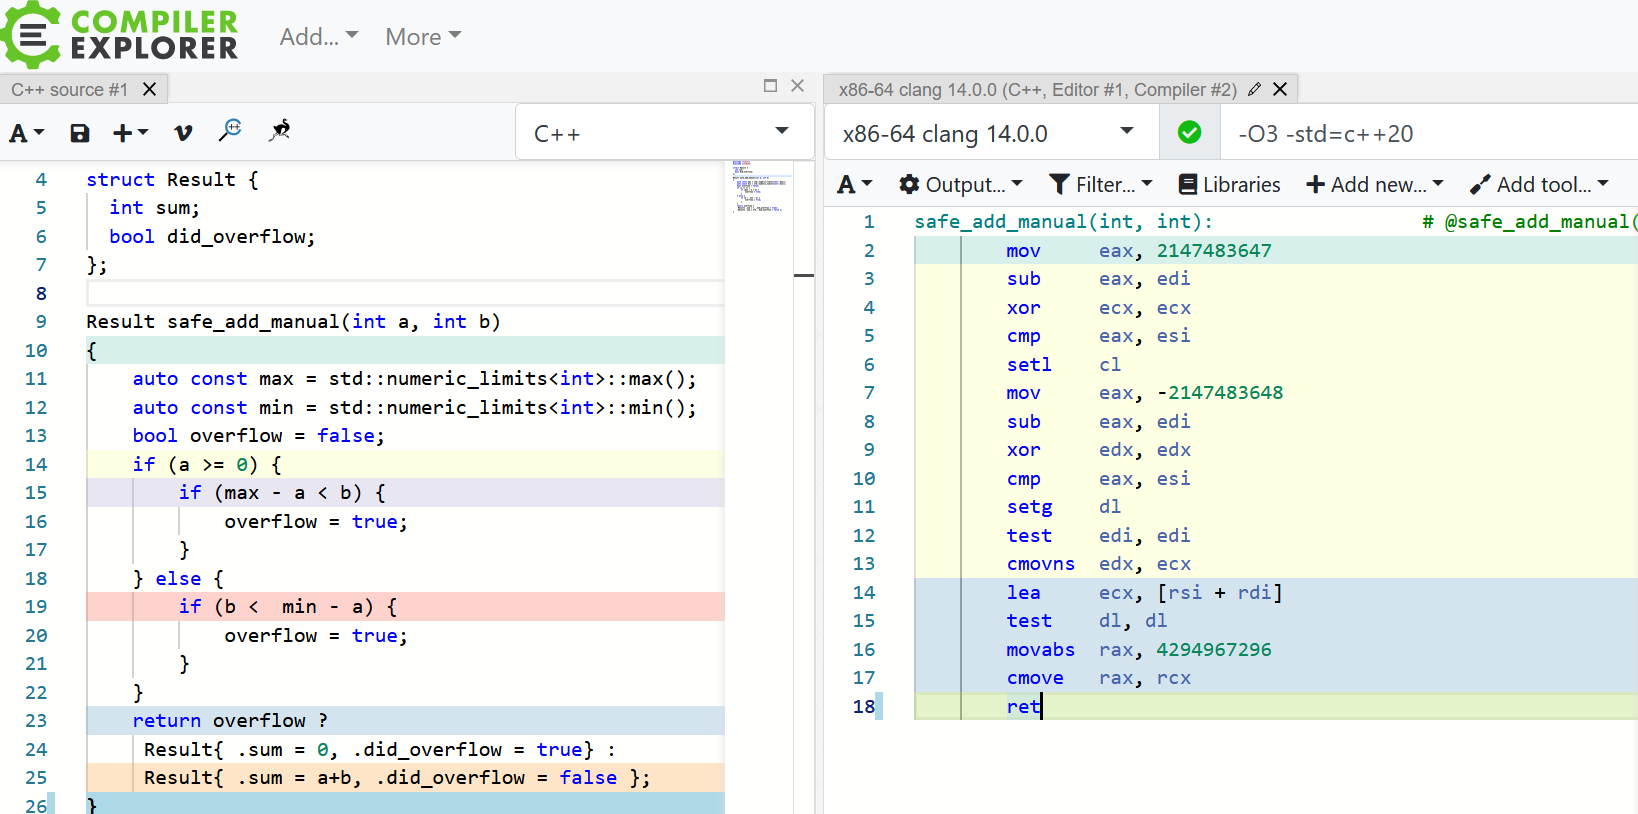
\includegraphics[width=.95\textwidth]{arithgfx/add_cpp_overflow.png}
\end{frame}

\begin{frame}
  \frametitle{Attempt \#1: Rely on the compiler to optimize it for us}

  \begin{itemize}
    \item The compiler does a bad job at detecting common patterns for overflow checking  \iftransitions \pause \fi 
    \item Also does a bad job at detecting double-width multiplication  \iftransitions \pause \fi 
    \item The only common optimization is double-width division  \iftransitions \pause \fi 
    \item Decent results for overflow checking can be obtained by using compiler-specific builtins  \iftransitions \pause \fi 
    \item It seems unlikely that this will change in the future, as it is a complex optimization for an uncommon use case
  \end{itemize}
\end{frame}

\begin{frame}[fragile]
  \frametitle{Attempt \#2: Write it in assembly}

  \iftransitions \pause \fi
  Naïve assembly implementation providing checked addition functions
  
  \begin{lstlisting}
--------------------------------------------------------
Benchmark                  Time         CPU   Iterations
--------------------------------------------------------
BM_lines32             83726 ns    71875 ns        10000
BM_linesWrapped32     167299 ns   154164 ns         3446
BM_linesSafe32        551233 ns   544085 ns         1120
  \end{lstlisting}
  
  \begin{itemize}
  \item \texttt{Wrapped32} calls assembly functions but ignores the overflow flag returned
  \item \texttt{Safe32} adds C++ code to check for and propagate overflow errors. On overflow this type transitions to a sticky invalid state.
  \end{itemize}

\end{frame}

\begin{frame}
  \frametitle{Attempt \#2: Write it in assembly}
  
  Negative performance impacts
  \begin{itemize}
  \item Function call instruction overhead  \iftransitions \pause \fi 
  \item Bad caching behavior  \iftransitions \pause \fi 
  \item Register pressure on caller side  \iftransitions \pause \fi 
  \item Zero optimization opportunities for the compiler  \iftransitions \pause \fi 
  \item No, link-time optimizations don't help either  \iftransitions \pause \fi 
  \end{itemize}
  
  \vspace{20pt}
  This approach gets the job done, but the resulting code is far from ideal.
  Not really suitable as a building block for libraries.
\end{frame}

\begin{frame}
  \frametitle{Possible Solution: Standard Library Extension}
  
  \begin{itemize}
  \item Standard library functions are not ordinary functions  \iftransitions \pause \fi 
  \item Compilers may use special knowledge to apply optimizations  \iftransitions \pause \fi 
  \item A lot of this is already being provided through compiler-specific builtins, so it is standardizing existing practice
  \end{itemize}
\end{frame}

\begin{frame}[fragile]
  \frametitle{WG14 - N2683 \& N2792}
  
  N2683 - Towards Integer Safety (David Svoboda)
  
  \begin{lstlisting}
bool ckd_add(int_type1 *result,
             int_type2 x, int_type3 y);
  \end{lstlisting}
  
  \begin{itemize}
    \item If the function returns \texttt{false}, an overflow occurred  \iftransitions \pause \fi 
    \item Otherwise, \texttt{result} contains the correct sum  \iftransitions \pause \fi 
    \item Function is specified as being carried out in infinite precision arithmetic  \iftransitions \pause \fi 
    \item C wants to implement this with macros  \iftransitions \pause \fi 
    \item Only addresses overflow, not double-width operations
  \end{itemize}
\end{frame}

\begin{frame}[fragile]
  \frametitle{WG21 - SG6}
  
  P0103 - Overflow-Detecting and Double-Wide Arithmetic Operations (Lawrence Crowl)
  
  \begin{lstlisting}
template<typename T>
bool overflow_add( T* result, T a, T b );
template<typename T>
D(T) wide_mul( T a, T b );
  \end{lstlisting}

  \iftransitions \pause \fi 
  \begin{itemize}
  \item Adds functions for splitting and joining wide results  \iftransitions \pause \fi 
  \item Adds special fused operations for multi-word arithmetic (\texttt{add2}, \texttt{muladd})  \iftransitions \pause \fi 
  \item Covers a very extensive range of operations  \iftransitions \pause \fi 
  \item Now covered by P1889 Numerics Work In Progress
  \end{itemize}
\end{frame}

\begin{frame}[fragile]
  \frametitle{WG21 - SG6}
  
  P1619 - Functions for Testing Boundary Conditions on Integer Operations (Lisa Lippincott)
  
  \begin{lstlisting}
template <class A, class B>
bool can_add(A a, B b) noexcept;
template <class A>
bool can_promote_modular(A a) noexcept;
  \end{lstlisting}
  
  \begin{itemize}
  \item Extensive list of functions for checking whether an operation is safe  \iftransitions \pause \fi 
  \item Mostly useful for checking and expressing contracts, probably not so much for algorithm implementations
  \end{itemize}
\end{frame}

\begin{frame}[fragile]
  \frametitle{Caveats of library solutions}
  
  \begin{itemize}
    \item Bound to the calling conventions of the target platform?
  \end{itemize}
  \begin{lstlisting}
bool overflow_add(T* result, T a, T b);
// vs.
optional<T> overflow_add(T a, T b);
  \end{lstlisting}  \iftransitions \pause \fi 
  \begin{itemize}
    \item We absolutely do not want these to incur full function call overhead  \iftransitions \pause \fi
    \item Should be implemented as a compiler builtin (intrinsics), but the standard cannot enforce that
  \end{itemize}
\end{frame}

\begin{frame}
  \frametitle{Sufficient Room for Core Language Extension?}
  
  \iftransitions \pause \fi 
  \begin{itemize}
    \item Because compilers already have special knowledge about standard library functions, this is probably not needed for optimal codegen \iftransitions \pause \fi 
    \item Even things that are hard to express in pure library form, compilers do a pretty good job already:
  \end{itemize}
  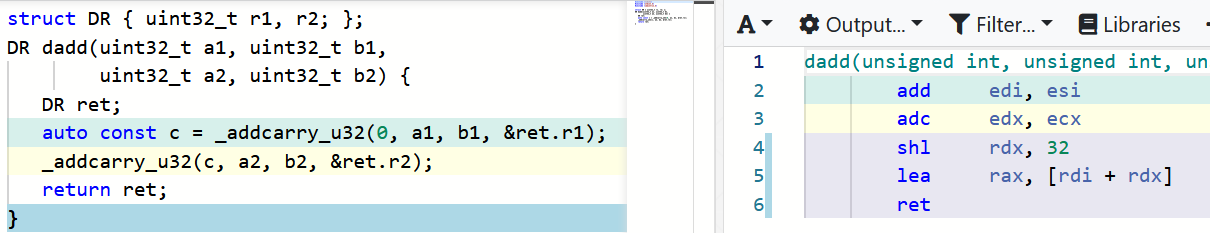
\includegraphics[width=.95\textwidth]{arithgfx/double_add.png}
\end{frame}


\begin{frame}
  \frametitle{Wrapping up\ldots}

  \begin{itemize}
  \item The fundamental building blocks for building advanced integer algorithms are given by the hardware
  \item Built-in integer types do a poor job at mapping to the hardware instructions
  \item Well established solutions exist in the field to allow more direct access to those instructions for advanced uses
  \item ISO C++ is behind other languages in adopting these solutions, but with the ongoing proposals has a good chance of catching up
  \end{itemize}
\end{frame}


\begin{frame}
\frametitle{References}

\begin{itemize}
  \item Harris \& Harris - Digital Design and Computer Architecture, 2nd Edition, Morgan Kaufmann 2013
  \item \href{https://www.open-std.org/jtc1/sc22/wg21/docs/papers/2018/p0907r4.html}{WG21 P0907 - Signed Integers are Two's complement}
  \item \href{http://standards.iso.org/ittf/PubliclyAvailableStandards/c051317_ISO_IEC_10967-1_2012.zip}{ISO/IEC 10967:1 (2012) - Language Independent Arithmetic: Integer and Floating Point Arithmetic}
  \item \href{https://www.open-std.org/jtc1/sc22/wg14/www/docs/n2683.pdf}{WG14 N2683 - Towards Integer Safety}
  \item \href{https://www.open-std.org/jtc1/sc22/wg14/www/docs/n2792.pdf}{WG14 N2792 - Supplemental Integer Safety}
  \item \href{https://www.open-std.org/jtc1/sc22/wg21/docs/papers/2017/p0103r1.html}{WG21 P0103R1 - Overflow-Detecting and Double-Wide Arithmetic Operations}
  \item \href{https://www.open-std.org/jtc1/sc22/wg21/docs/papers/2019/p1619r1.pdf}{WG21 P1619R1 - Functions for Testing Boundary Conditions on Integer Operations}
\end{itemize}

\end{frame}


\begin{frame}
  \frametitle{Thanks for your attention.}

  \href{https://stackoverflow.com/users/577603/comicsansms}{
\includegraphics[height=.05\textheight]{resources/so-icon.png}}
  \href{https://github.com/ComicSansMS}{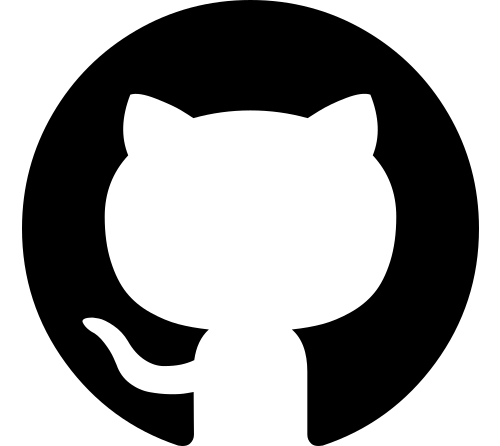
\includegraphics[height=.05\textheight]{resources/github-icon.png}}
  \includegraphics[height=.05\textheight]{resources/discord-icon.png} ComicSansMS /
  \href{https://twitter.com/DerGhulbus/}{
\includegraphics[height=.05\textheight]{resources/twitter-icon.png} @DerGhulbus}
\end{frame}


\iffalse
\begin{frame}
  \frametitle{Calculating with Rational numbers}
  
  \begin{equation*}
  \begin{split}
  \sin x = x - \frac{x^3}{3!} + \frac{x^5}{5!} - \frac{x^7}{7!} + \frac{x^9}{9!} - \ldots \\
  = \sum_{n = 0}^{\infty}{(-1)^n \frac{x^{2n+1}}{(2n+1)!}}
  \end{split}
  \end{equation*}
  
  \begin{equation*}
  \begin{split}
  e^x = 1+ x + \frac{x^2}{2!} + \frac{x^3}{3!} + \frac{x^4}{4!} + \ldots \\
  = \sum_{n = 0}^{\infty}{\frac{x^{n}}{n!}}
  \end{split}
  \end{equation*}
\end{frame}
\fi

\end{document}
